\documentclass[final]{thesis} %% Print thesis with figures!
%\documentclass[draft]{thesis} %% Print thesis without figures!

% This template uses biblatex for generating a list of references!

%----------------------------------------------------------------------------------------
% METATEXT FOR THE PDF-FILE
%----------------------------------------------------------------------------------------
\hypersetup{%
	pdftitle    = {Thesis},% <-- Change here the title of your thesis
	pdfauthor   = {Antero Voutilainen},% <-- Change here your full name i.e. first name and last name
	pdfsubject  = {Master's Thesis},% <-- Change here the type of your thesis
	pdfproducer = {pdfTeX} % <-- Change here the name of the pdf-converted if known
}

%----------------------------------------------------------------------------------------
% FORMATTING COMMANGS FOR THE BIBLIOGRAPHY GENERATED WITH BibLaTeX:
%----------------------------------------------------------------------------------------
\usepackage{csquotes}
\usepackage[backend=biber,style=numeric-comp,sorting=none,maxnames=3,minnames=1,giveninits=true]{biblatex}
\DefineBibliographyStrings{finnish}{%
    andothers  = {ym.},%
    references = {Lähteet},%
    mathesis   = {pro gradu~-tutkielma},%
    phdthesis  = {väitöskirja}
}
\addbibresource{lahteet.bib}%----------------------------------------------------------------------------------------
% CONTENT OF THE TITLEPAGE - 
% Change the title, author, supervisor(s), thesis type and the date when you submit your 
% thesis for evaluation.
%----------------------------------------------------------------------------------------

\title{Rapid proton capture process in type I X-ray bursts generated in LMXBs with the effects of nuclear masses}
\author{Antero Voutilainen}
\supervisor{Anu Kankainen\\Miikka Winter}
\project{Master's Thesis}
\date{\today}

%----------------------------------------------------------------------------------------
% ADDITIONAL TEX-PACKAGES 
%----------------------------------------------------------------------------------------
\usepackage{amsmath}
\usepackage{amsfonts}
\usepackage{amssymb}
\usepackage{comment}
\usepackage{svg}
\usepackage[final]{pdfpages}
\usepackage{float}
\usepackage{empheq}
\usepackage{tikz}

%----------------------------------------------------------------------------------------
% MAIN DOCUMENT
%----------------------------------------------------------------------------------------
\begin{document}
%----------------------------------------------------------------------------------------
% PRINT TITLEPAGE WITH THE FOLLOWING COMMAND
%----------------------------------------------------------------------------------------
\titleJYFL


%----------------------------------------------------------------------------------------
%	ABSTRACT
%----------------------------------------------------------------------------------------
\section*{Abstract}
\addcontentsline{toc}{section}{Abstract}

% Bibliographic information
\begin{singlespace}
	Voutilainen, Antero\\
	Rapid proton capture process in type I X-ray bursts generated in LMXBs with the effects of nuclear masses \\
	Master’s thesis \\
	Department of Physics, University of Jyväskylä, 2025, \pageref{LastPage}~pages.
\end{singlespace}

\bigskip

\begin{comment}
% Abstract text
\noindent This should be written in English. \lipsum[1]
\end{comment}

\bigskip 

% Keywords
\noindent Keywords: Thesis, abstract, writing, instructions

%----------------------------------------------------------------------------------------
% ABSTRACT IN FINNISH (COMPULSORY FOR ALL)
%----------------------------------------------------------------------------------------
\section*{Tiivistelmä}
\addcontentsline{toc}{section}{Tiivistelmä}

% Bibliografiset tiedot
\begin{singlespace}
	Voutilainen, Antero\\ 
	Rapid proton capture process in type I X-ray bursts generated in LMXBs with the effects of nuclear masses\\
	Pro gradu~-tutkielma\\ 
	Fysiikan laitos, Jyväskylän yliopisto, 2025, \pageref{LastPage}~sivua
\end{singlespace}

\bigskip

% Tiivistelmän teksti
\begin{otherlanguage}{finnish}


\begin{comment}
\noindent Heti opinnäytteen nimiölehden jälkeen sijoitettava tiivistelmä on yhdelle paperille mahtuva ja tavallisesti enintään 250 sanaa sisältävä yhteenveto, joka hyvin tiiviissä muodossa informoi kirjoituksesta. On tärkeää, että tiivistelmä laaditaan huolellisesti, koska sen välityksellä tieto kirjoituksesta leviää eri tietokantojen kautta. Sen tulee olla laadittu niin, että se sellaisenaan voidaan julkaista tietokannoissa. Tiivistelmään alkuun on merkittävä opinnäytteen bibliografiset tiedot ja sen lopussa mainitaan sitä kuvaavat avainsanat. Tiivistelmiä on kahta tyyppiä. Informatiivinen tiivistelmä on tärkein. Se kertoo, mitä ja miten on tutkittu ja mitkä ovat tulokset. Indikatiivinen tiivistelmä osoittaa, mitä kirjoituksessa on käsitelty. Se on sisällöltään yleisempi kuin informatiivinen tiivistelmä, eikä se kerro tuloksista. Tiivistelmän loppuun liitetään aihetta kuvaavat 3--5 avainsanaa helpottamaan tietokantajärjestelmien työtä. Avainsanat voidaan antaa vapaasti asiasisällön mukaan tai poimia termit alan kontrolloiduista sanastoista kuten Yleisestä suomalaisesta asiasanastosta YSA. Opinnäytteen tunnistamiseksi tarvittavat bibliografiset tiedot annetaan tiivistelmän alussa. Tarvittavat tiedot ovat kirjoittajan suku- ja etunimi, opinnäytteen otsikko, opinnäytteen tyyppi, ainelaitoksen nimi, yliopiston nimi, valmistumisvuosi ja työn sivujen lukumäärä (ilman liitesivuja).
\end{comment}
\end{otherlanguage}

\bigskip

% Avainsanat
\noindent Avainsanat: Opinnäyte, tiivistelmä, kirjoittaminen, ohjeet

% --------------------------------------------------------------------------
% PREFACE
% --------------------------------------------------------------------------
\section*{Preface}
\addcontentsline{toc}{section}{Preface}

\begin{comment}

Esipuheen teksti tulee tähän. \lipsum[1]

\end{comment}

\bigskip

\noindent Jyväskylä January 1, 2020

\bigskip

\noindent Olli Opiskelija

% --------------------------------------------------------------------------
% TABLE OF CONTENTS
% --------------------------------------------------------------------------
\tableofcontents

% --------------------------------------------------------------------------
% MAIN TEXT
% --------------------------------------------------------------------------
\section{Introduction}
\label{sec:introduction}


\begin{comment}
Johdannon tehtävänä on nimensä mukaisesti johdatella lukija käsillä olevan tutkimuksen maailmaan. Tutkiminen ja kirjoittaminen kuuluvat yhteen. Tutkimus on monella alalla, varsinkin niin sanotuissa ihmistieteissä, pelkistetysti sanottuna kirjoitusprosessi. Sen päämäärä on ajattelun tulos, kirkastunut ydin niistä ajatuksista ja johtopäätöksistä, joita prosessin aikana on syntynyt. Kirjoittaminen jäsentää ajattelua ja synnyttää uusia ideoita. Siksi kirjoittaminen on olennainen osa sekä opiskelua, tutkimusta että lopulta myös ammattitaitoa. Kirjoitustaitoa tarvitaan läpi työelämän: lähes kaikissa akateemisissa ammateissa laaditaan muistioita, virkakirjeitä, raportteja, tiedotteita tai suunnitelmia.

Kielijelpin kirjoitusviestinnän sivuilla keskitytään tieteellisen kirjoittamisen perusasioihin, kirjoitusprosessiin ja tekstin viimeistelyyn. Kielijelppi lähestyy tieteellistä kirjoittamista laadullisen tutkimuksen näkökulmasta, koska Kielijelpin kirjoitusviestinnän tekijöiden tausta ja kokemus ovat laadullisen humanistisen tutkimuksen parissa. Sivustosta on toivottavasti kuitenkin iloa myös muunlaista tutkimusta tekeville.

\lipsum[1]
\end{comment}


\section{Theoretical background}
\label{sec:theory-background}


\subsection{Low Mass X-ray Binaries}
\label{subsec:lmxbs}

\subsubsection{Nuclear reaction network}
\label{subsec:nrn}

\subsubsection{Rapid Proton Capture Process}
\label{subsec:rpprocess}

\subsubsection{Total Reaction Rate}
\label{subsec:trr}

\subsubsection{Light Emission Curves}
\label{subsec:lec}


\subsection{TALYS}
\label{sec:talys}

\subsubsection{Hauser-Feshbach statistical model}
\label{subsec:HFsm}

\subsubsection{Parameters}
\label{subsec:tparams}


\subsection{Winnet}
\label{sec:winnet}

\section{Methods and materials}
\label{sec:methods-and-materials}




\section{Results}
\label{sec:results}

% Tulokset esittelee ja kommentoi tutkimuksen tuloksia normaalisti tutkimusongelmien esittämisjärjestyksessä.

% \begin{table}[h]
%    \centering
%    \caption{Selkeä hinnasto}
%    \begin{tabular}{llr} \toprule
%       \multicolumn{2}{c}{Artikkeli} \\ \cmidrule(r){1-2}
%       Eläin    & Kuvaus       & hinta (mk) \\ \midrule
%       Hyttynen & grammoittain &  41,50 \\
%                & kappaleelta  &   0,05 \\
							
%       Gnu      & täytetty     & 360,00 \\
%       Emu      & täytetty     & 121,30 \\
%       Vyötiäinen & pakastettu &  38,40 \\ \bottomrule
%    \end{tabular}
% \end{table}

% \begin{figure}[htp]
%    \centering
%    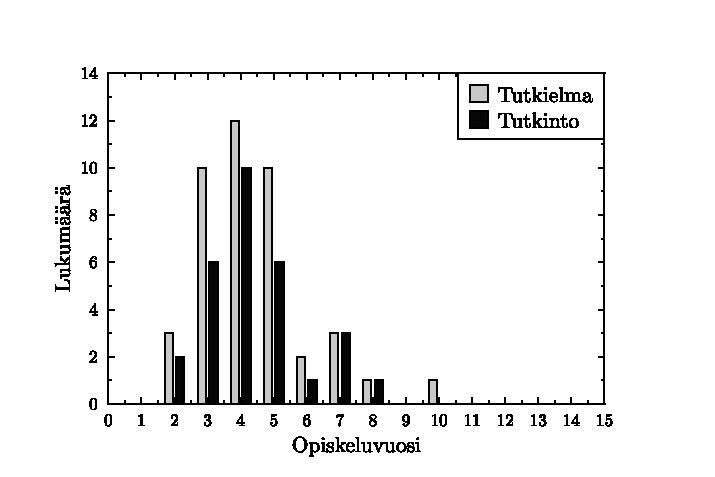
\includegraphics[width=\textwidth]{mallikuvio.pdf}
%    \caption{Valmistuneiden kandidaatintutkielmien jakauma tekijän opiskeluvuoden mukaan Jyväskylän yliopiston fysiikan laitoksella 2014 ($n = 42$); tutkintojen jakauma opiskeluvuoden mukaan, kun tutkielma on valmistunut 2014 ($n = 29$; tilanne 4.3.2015). (Kuva: Jussi Maunuksela, 2015)}
%    \label{fig:esim-kuvio}
% \end{figure}


\section{Conclusions}
\label{sec:conclusions}

% Loppuluvussa arvioidaan tutkimusta ja sen tuloksia. \lipsum[1]

\nocite{*}

% --------------------------------------------------------------------------
% REFERENCES
% --------------------------------------------------------------------------
\addcontentsline{toc}{section}{References}
\printbibliography

\newpage

% --------------------------------------------------------------------------
% APPENDICES
% --------------------------------------------------------------------------
\appendix

\section{First appendix}
\label{sec:first-appendix}

\lipsum[2-3]

\section{Second appendix}
\label{sec:second-appendix}

\lipsum[2-3]

\end{document}

